\documentclass[letterpaper, 11pt]{article}
%\usepackage[hmargin = 1in, vmargin = 1in]{geometry}
\usepackage{amsmath}
\usepackage{amssymb}
\usepackage{enumitem}
\usepackage{mathrsfs}
\usepackage{tikz}
\usepackage{graphicx}
\usepackage{algorithmicx}
\usepackage{algpseudocode}
\usepackage{mathtools}
\usepackage[linguistics]{forest}
% \doublespacing
\setlength{\headheight}{14pt}
\usepackage{fancyhdr}
\pagestyle{fancy}
\rhead{Gabriel Wallace}
\lhead{Comp Sci 3130}

\newcommand{\card}{\text{Card}}
\newcommand{\N}{\mathbb{N}}
\newcommand{\R}{\mathbb{R}}
\newcommand{\Z}{\mathbb{Z}}
\newcommand{\Q}{\mathbb{Q}}

\newcommand{\inv}{^{-1}}
\newcommand{\abs}[1]{\lvert #1 \rvert}
\newcommand{\hwnumber}[1]{\newpage \noindent\textbf{#1.} \smallskip}
\newcommand{\hwnumbersec}[3]{\newpage \noindent\textbf{#1.} Section #2 \##3 \smallskip}
\newcommand{\Mod}[1]{\ \mathrm{mod}\ #1}
\newcommand{\Alg}[1]{\medskip \noindent\textbf{ALGORITHM} \( #1 \)} 
\newcommand{\To}{\textbf{ to }}

\DeclarePairedDelimiter{\ceil}{\lceil}{\rceil}

\begin{document}

\hwnumber{1}

We want to multiply 2101 and 1130. We have 
\begin{align*}
  c_2 &= 21 * 11 \\
  c_0 &= 01 * 30 \\
  c_1 &= (21 + 01) * (11 + 30) - ((21 * 11) + 01 * 30)\\
      &= (22 * 41) - (21 * 11) - (01 * 30)
\end{align*}

Thus we break it down further as follows.

For \(21 * 11\) we have:
\begin{align*}
  c_2 &= 2 * 1 = 2 \\
  c_0 &= 1 * 1 = 1 \\
  c_1 &= (2 + 1) * (1 * 1) - (2 * 1 + 1 * 1)\\
      &= 3
\end{align*}
So 
\[21 * 11 = 2 \cdot 10^2 + 3\cdot 10 + 1 = 231\]

For \(01 * 30\) we have:
\begin{align*}
  c_2 &= 0 * 3 = 0 \\ 
  c_0 &= 1 * 0 = 0 \\
  c_1 &=  (0 + 1) * (3 + 0) - (0 + 0) \\
      &= 3
\end{align*}
So
\[01 * 30 = 0\cdot 10^2 + 3 \cdot 10 + 0 = 30\]

For \(01 * 30\) we have:
\begin{align*}
  c_2 &= 2 * 4 = 8 \\
  c_0 &= 2 * 1 = 2 \\
  c_1 &= (2 + 2) * (4 * 1) - (8 + 2)\\
      &= 10
\end{align*}
So 
\[22 * 41 = 8 \cdot 10^2 + 10 \cdot 10 + 2 = 902\]

Putting it all together, we have
\begin{align*}
  2101 * 1130 &= 231 \cdot 10^4 + (902 - 231 - 30) \cdot 10^2 + 30\\
              &= 2,374,130
\end{align*}

\hwnumber{2}

\begin{figure}[h!]
  \centering
  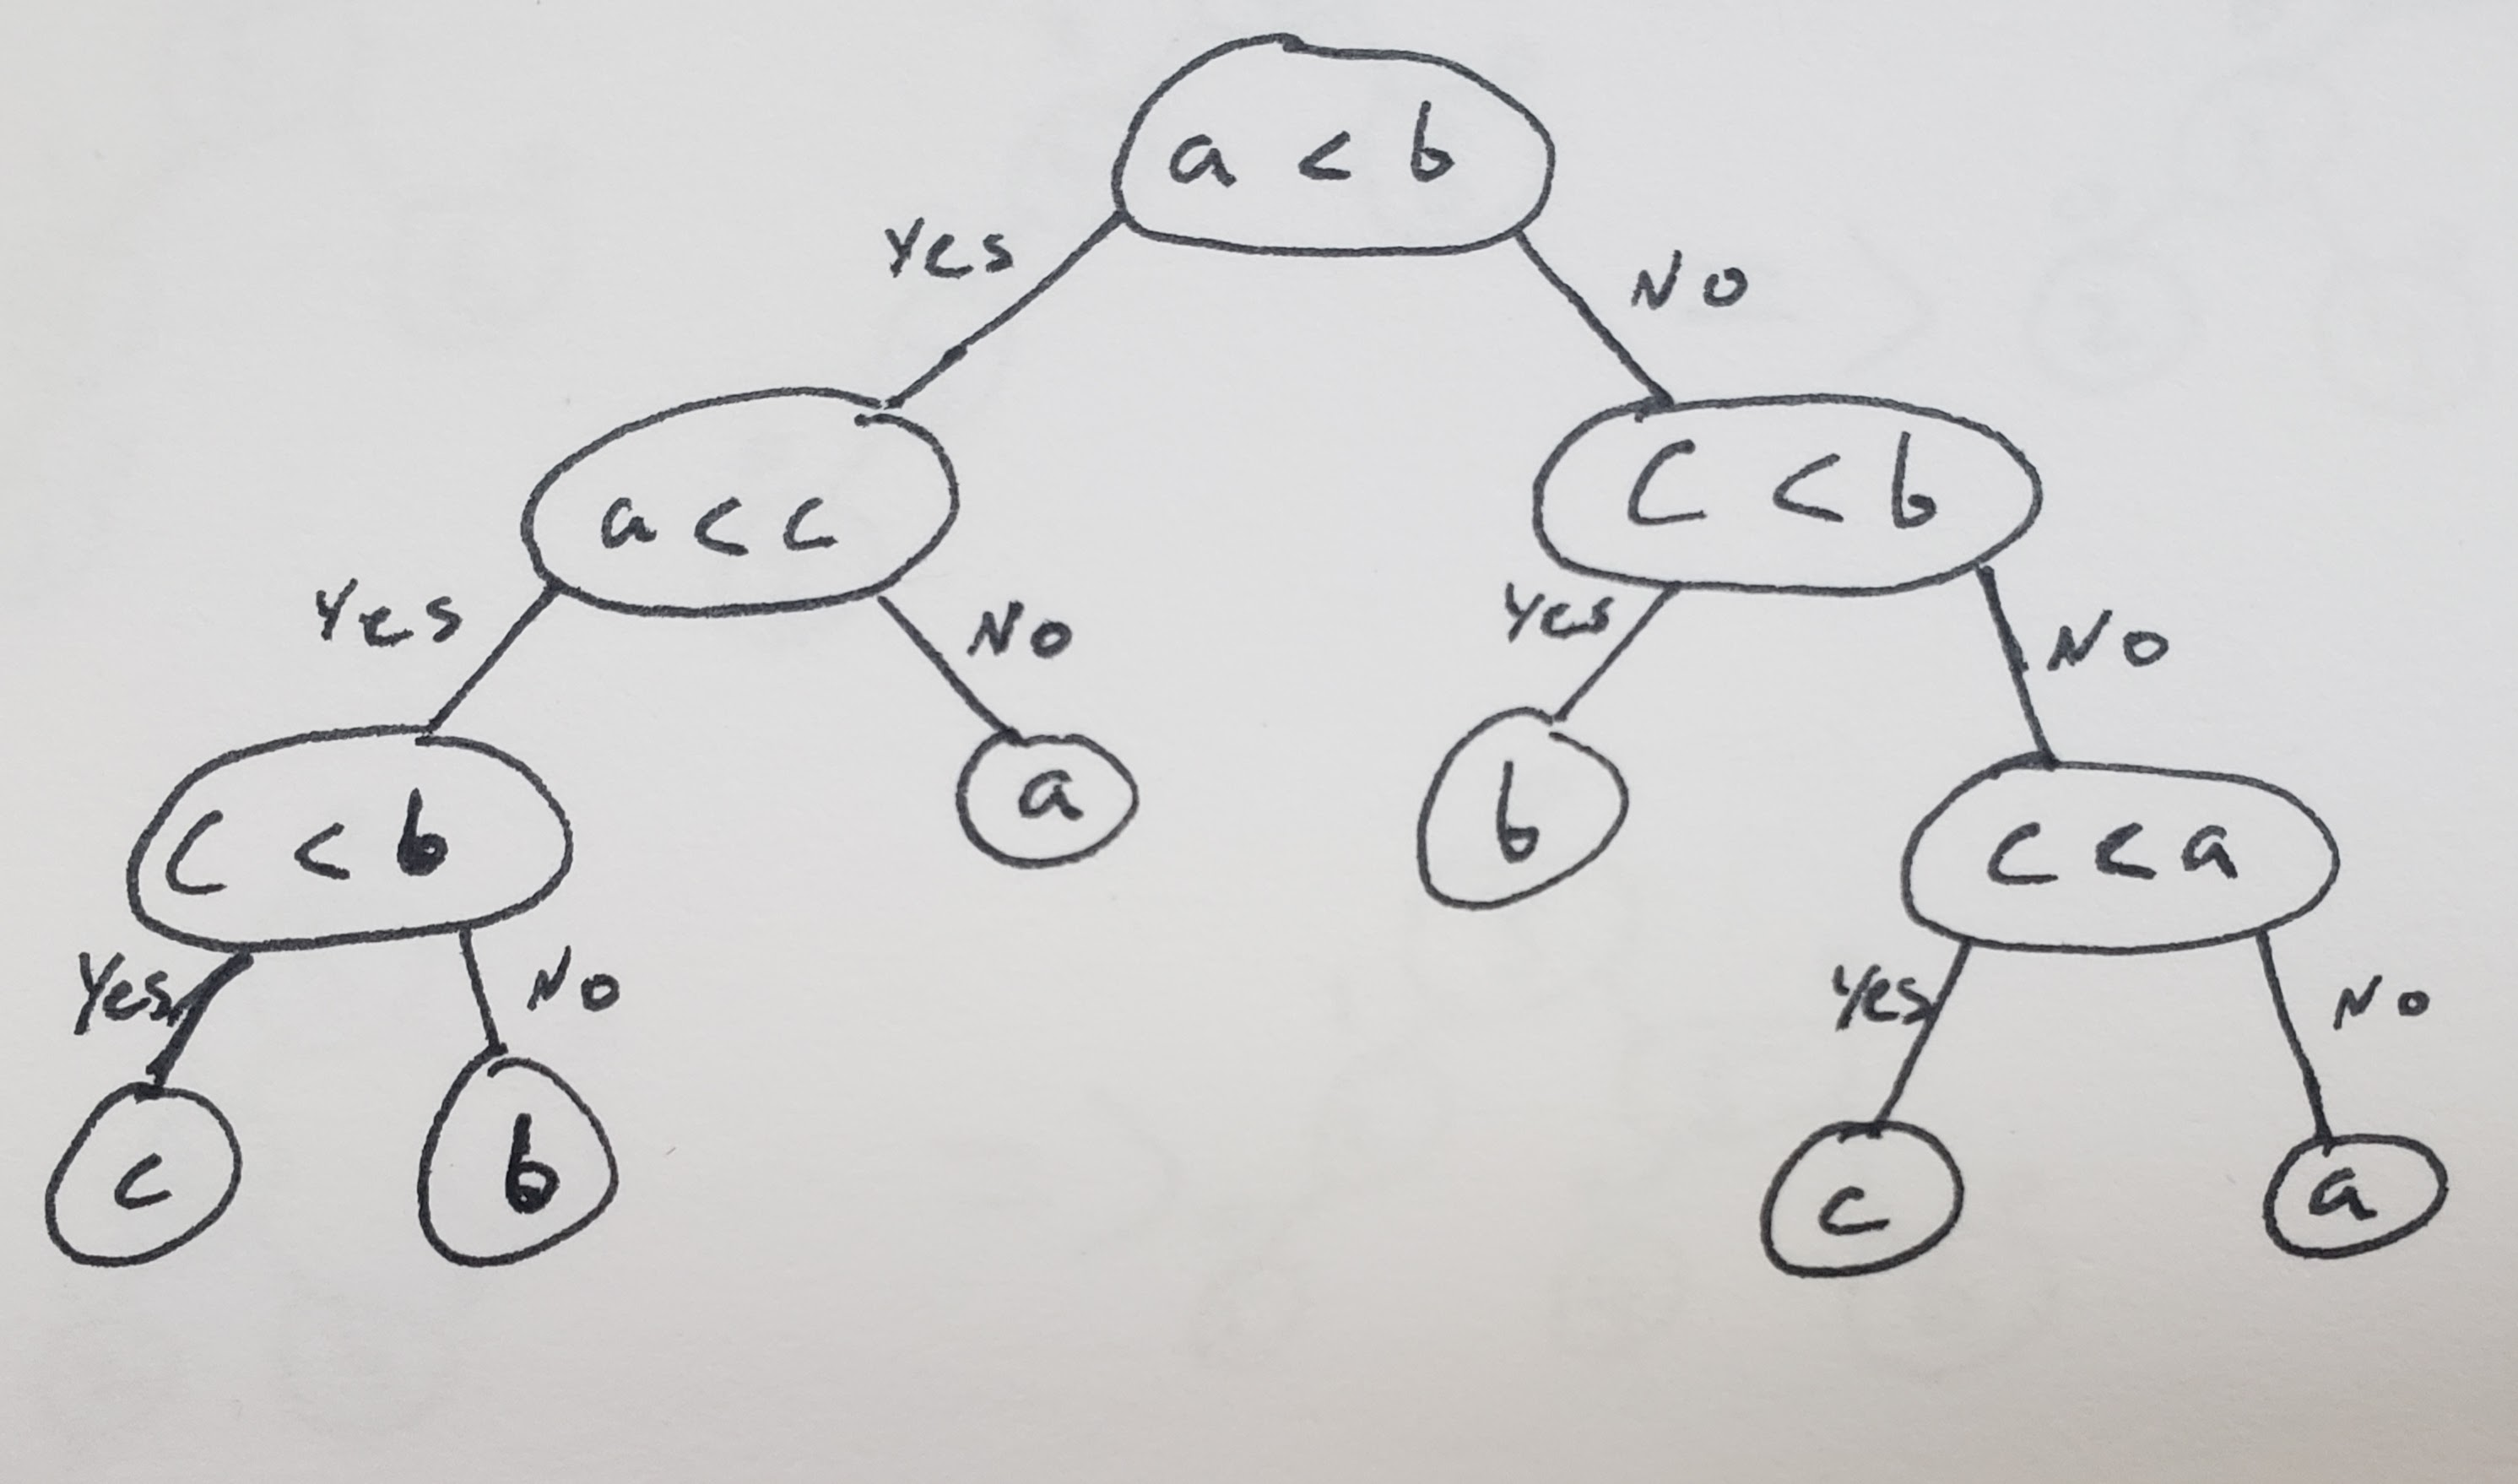
\includegraphics[width=\linewidth]{pics/num_2.jpg}
\end{figure}

\hwnumber{3}
\begin{enumerate}[label = (\alph*)]
  \item First we sort the array with a sorting algorithm with optimal
    efficiency will be in the first and last positions of the array
    respectively. Thus, we have an efficiency as follows:
    \[T(n) = T_{\text{sort}}(n) + T_{\text{select}}(n) \in \Theta(n\log n) +
    \Theta(1) = \Theta(n \log n)\]

  \item First assign a varible called \texttt{min} to \(A[0]\) and then loop
    through the array and if \(A[i]\) is less than \texttt{min}, then reassign
    \texttt{min} to \(A[i]\). Then create a variable called \texttt{max} and
    loop through again reassigning if an element of the array is larger than
    \texttt{max}. Since we had to loop through the array twice, then \(T(n) =
    2n\) and \(T(n) \in \Theta(n)\).
\end{enumerate}

\newpage
\hwnumber{4 (b)}
\begin{figure}[h!]
  \centering
  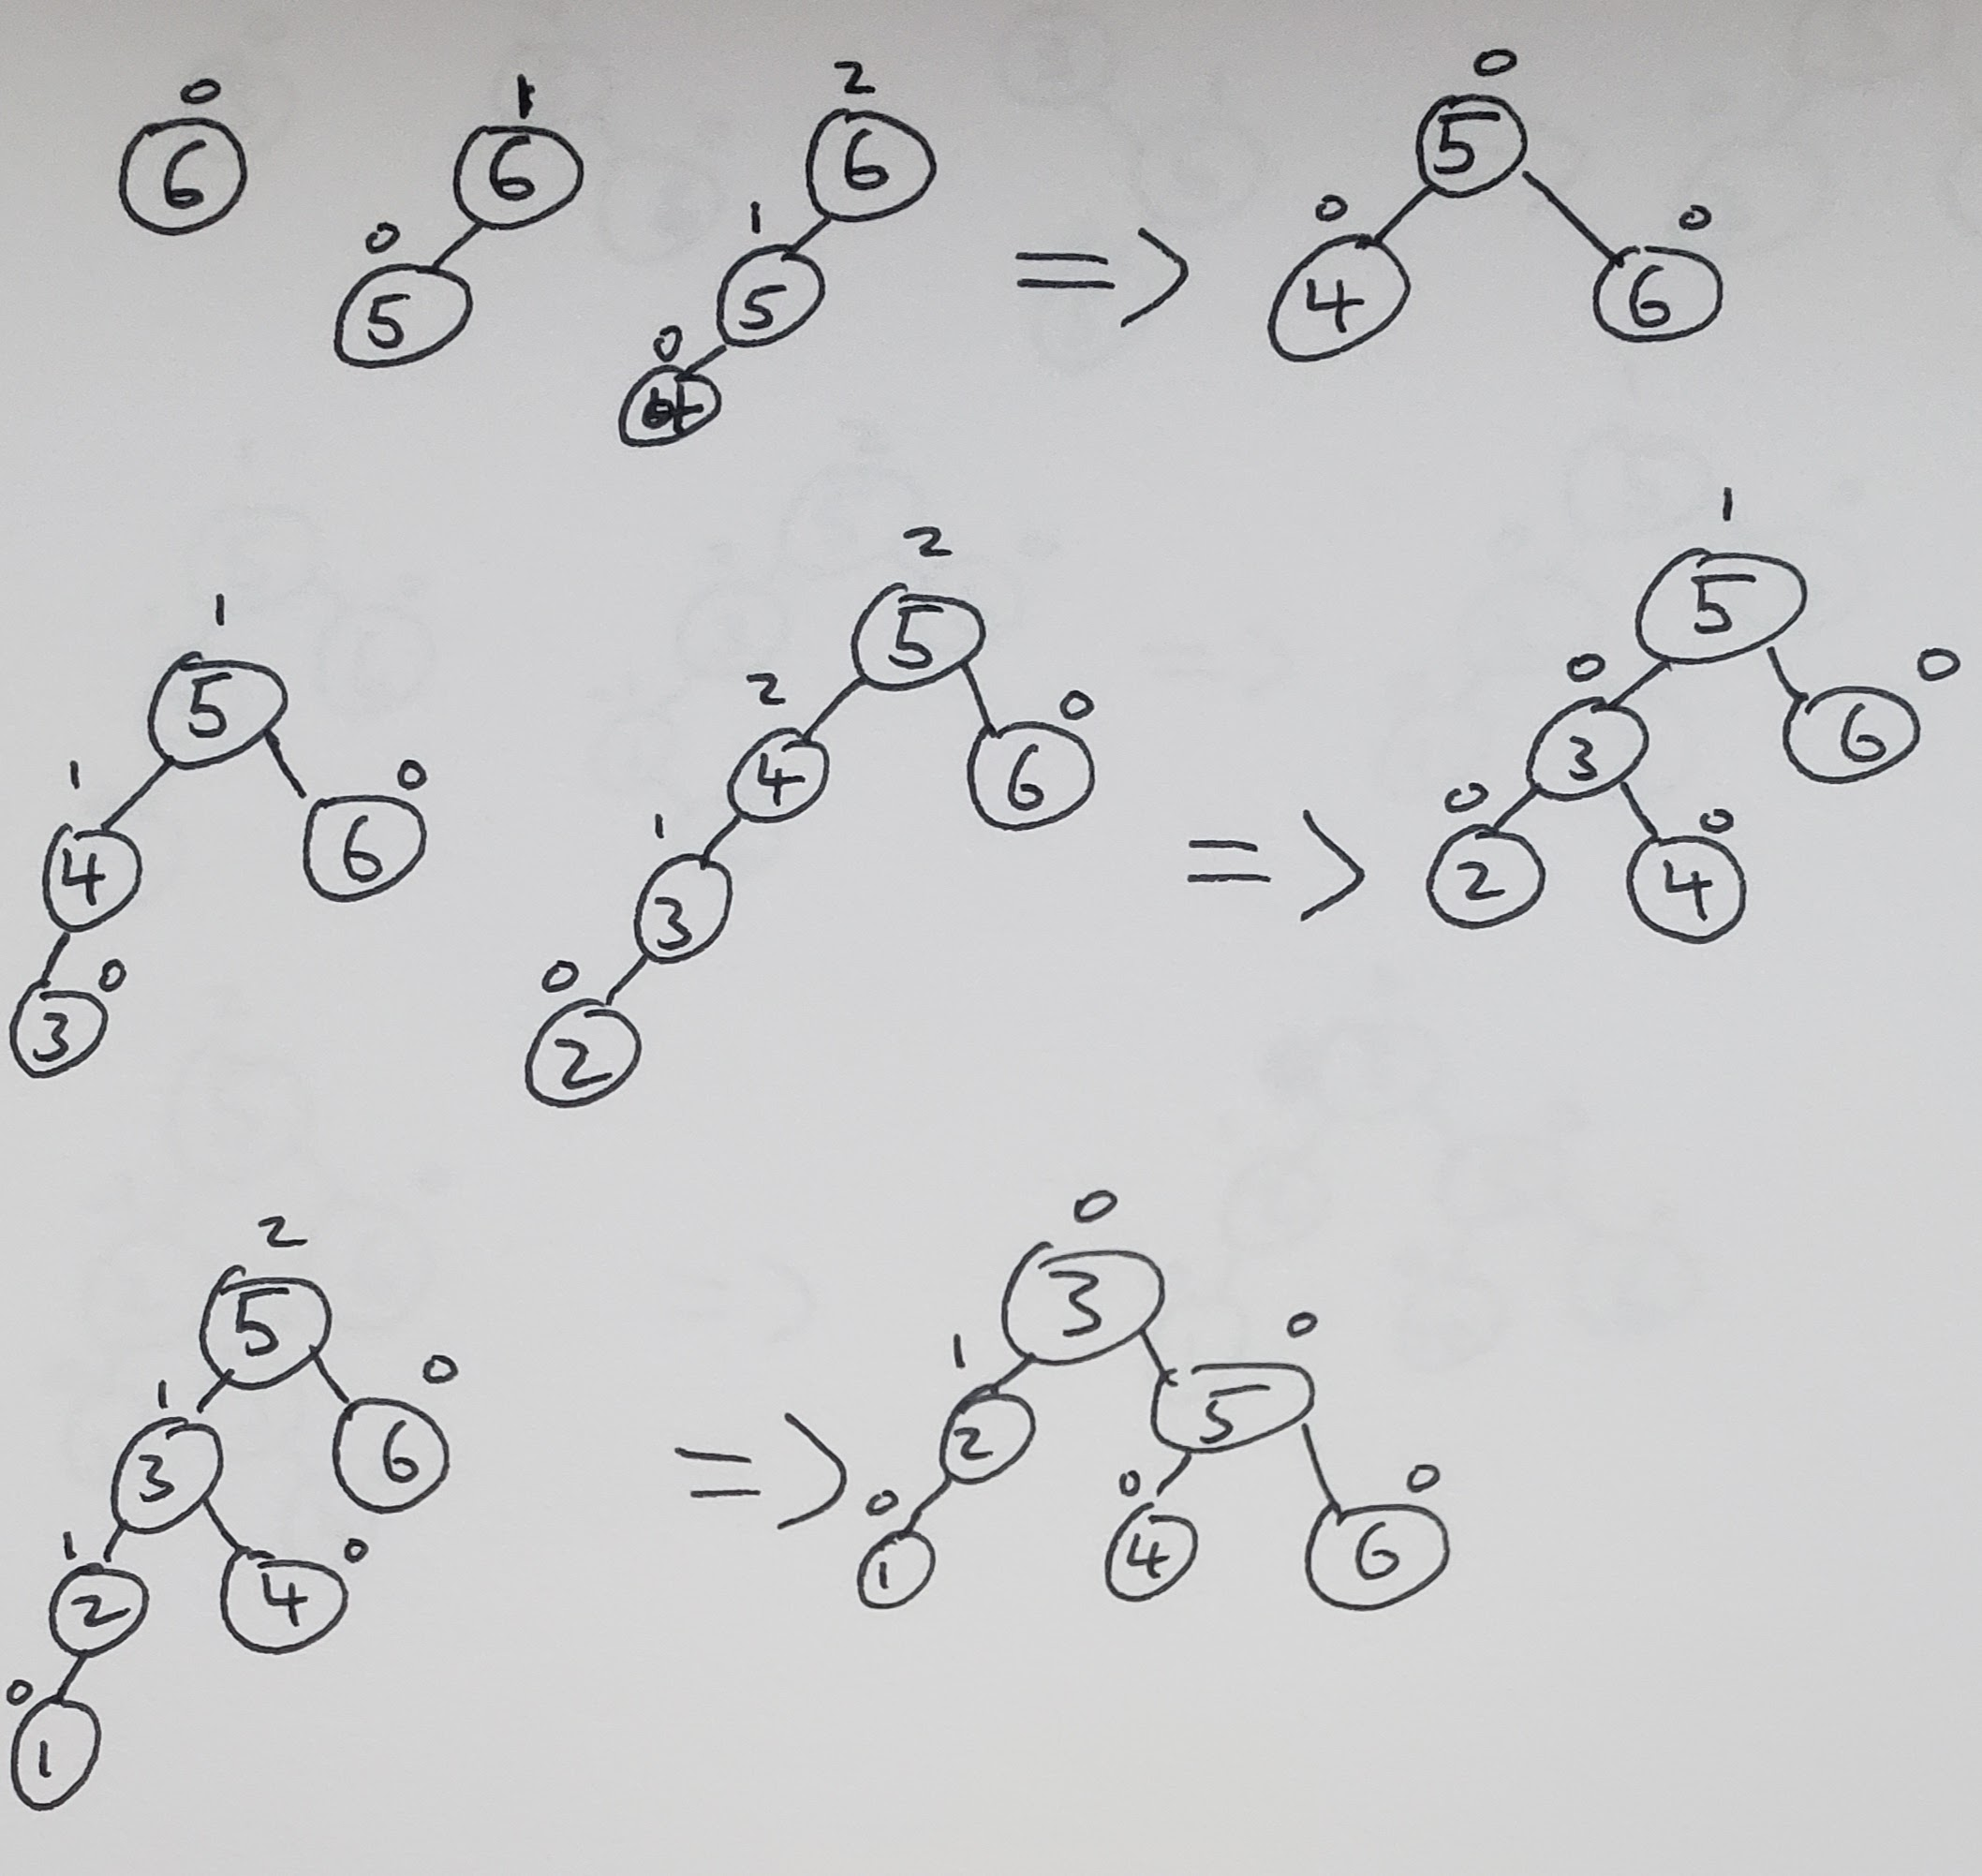
\includegraphics[width=\linewidth]{pics/num_4.jpg}
\end{figure}

\hwnumber{4 (c)}
\begin{figure}[h!]
  \centering
  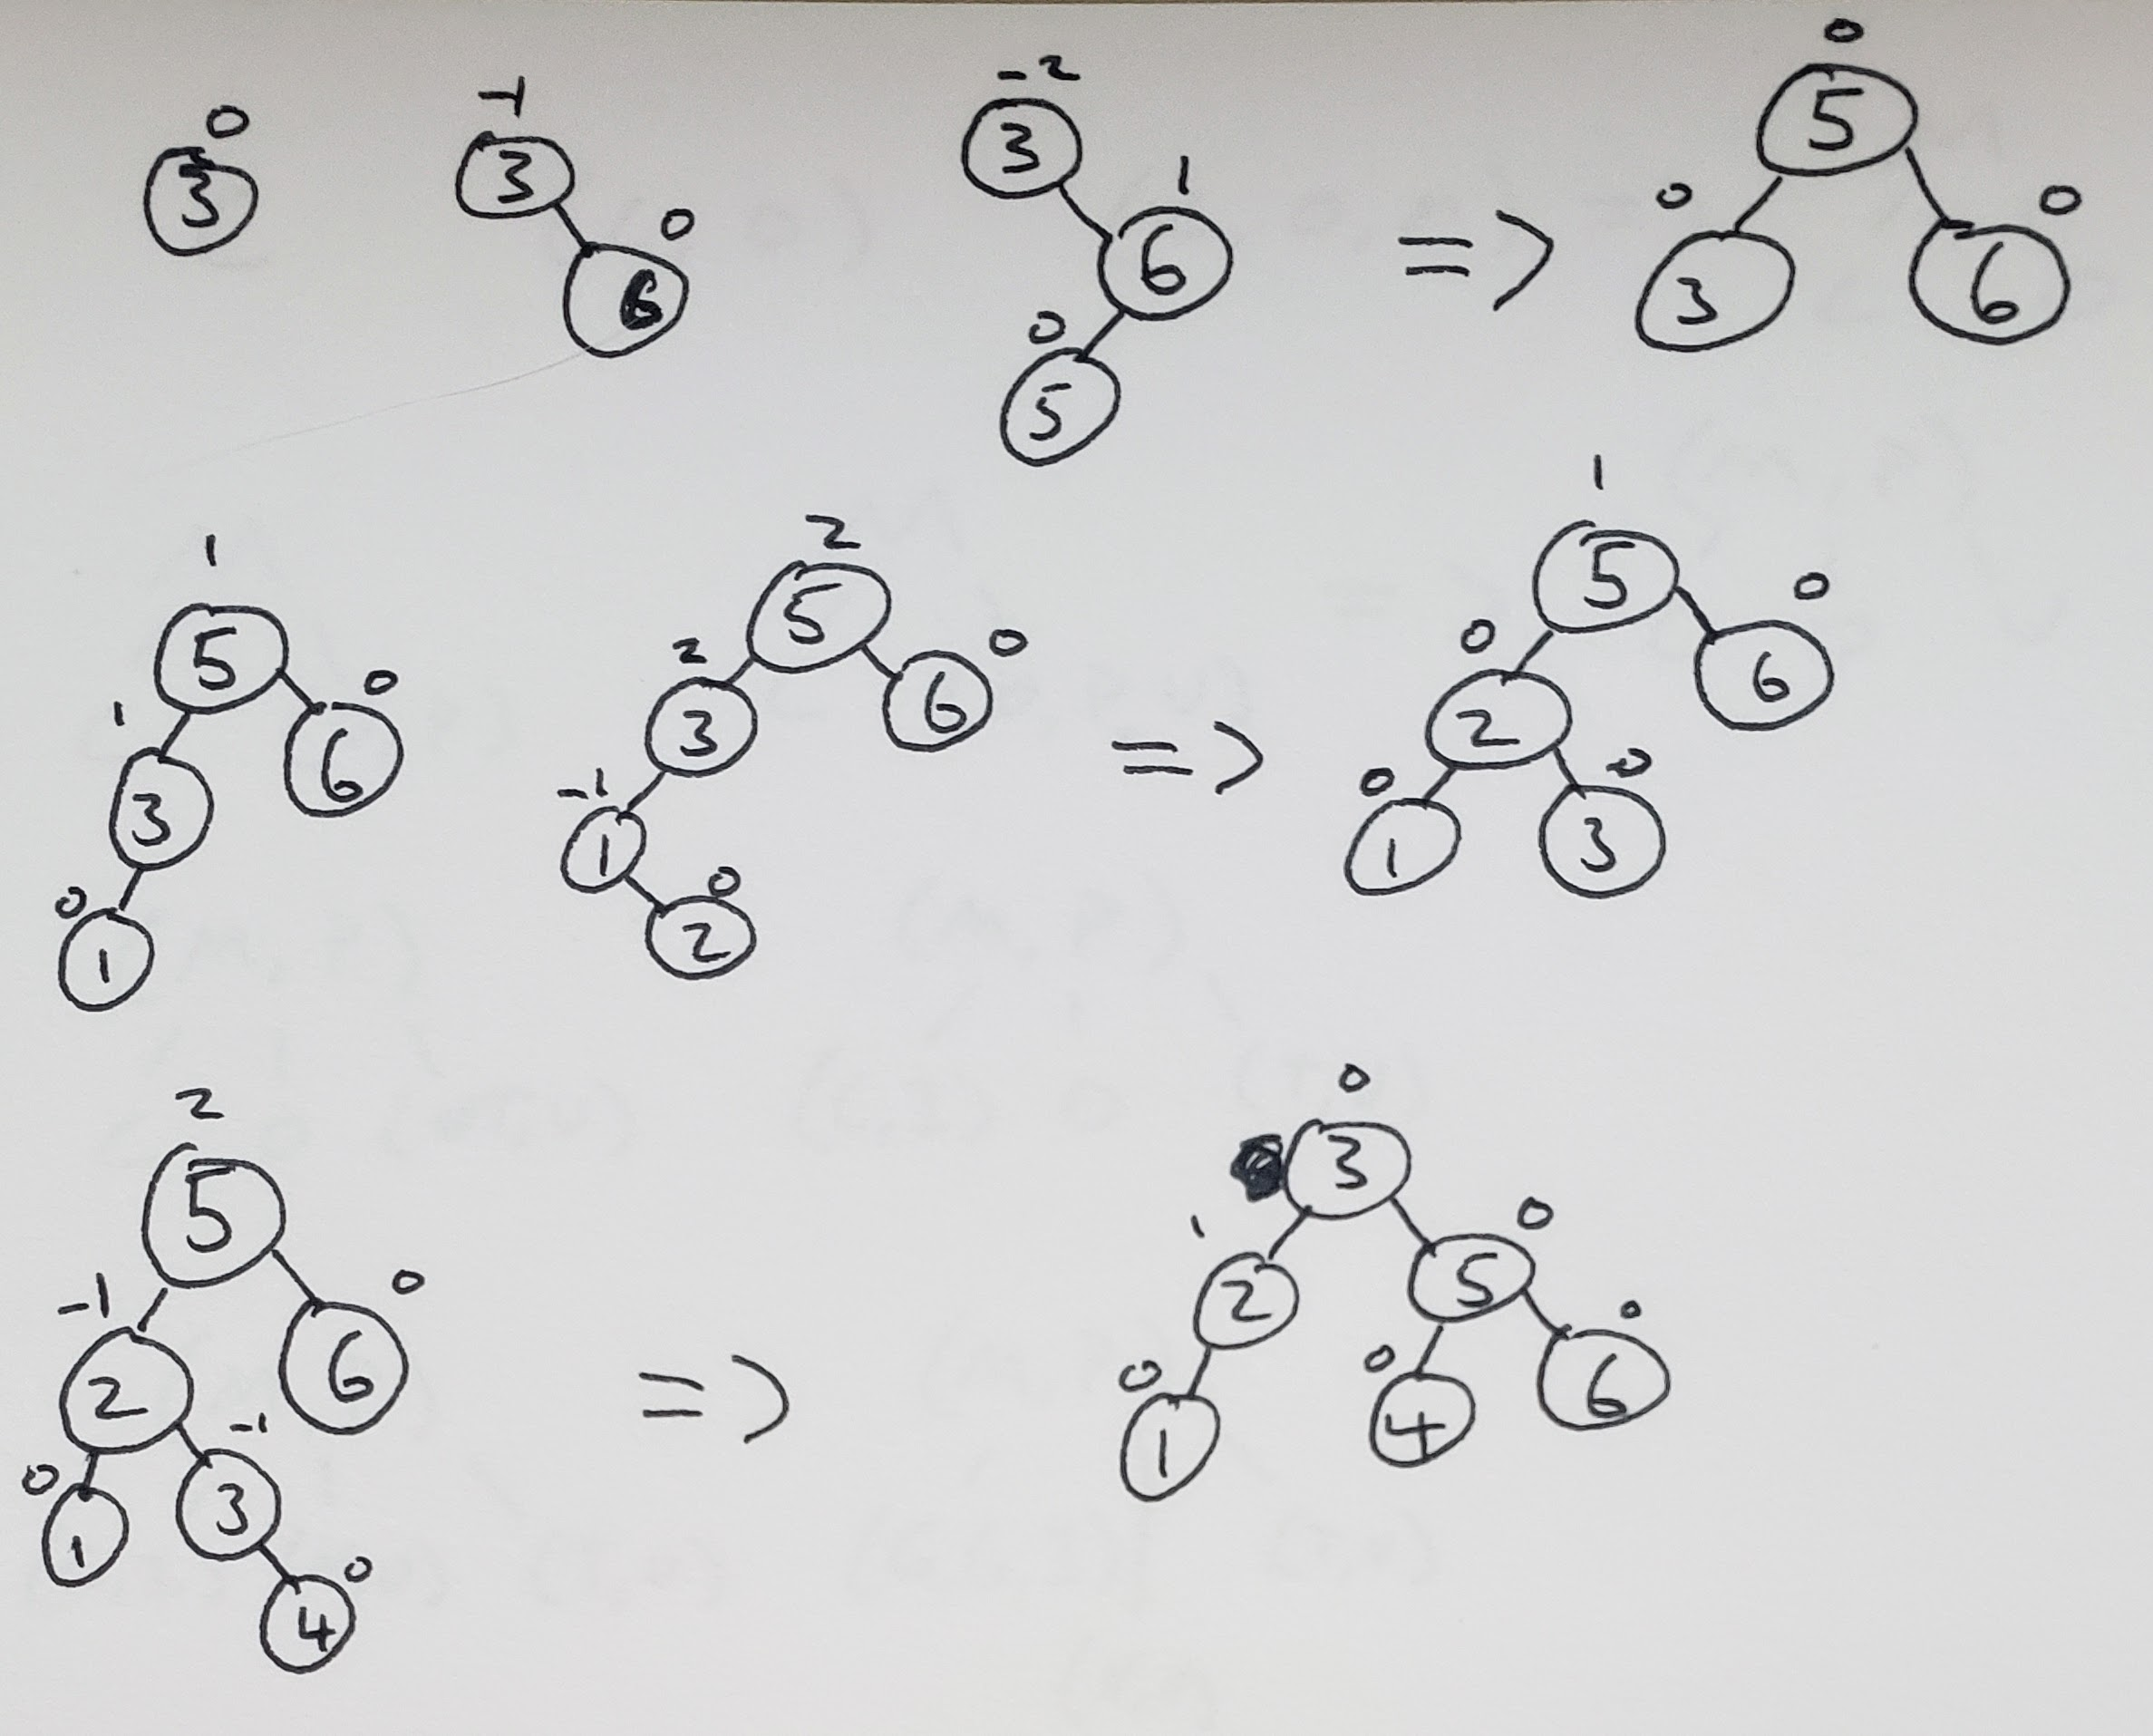
\includegraphics[width=\linewidth]{pics/num4_c.jpg}
\end{figure}

\hwnumber{5}
\begin{figure}[h!]
  \centering
  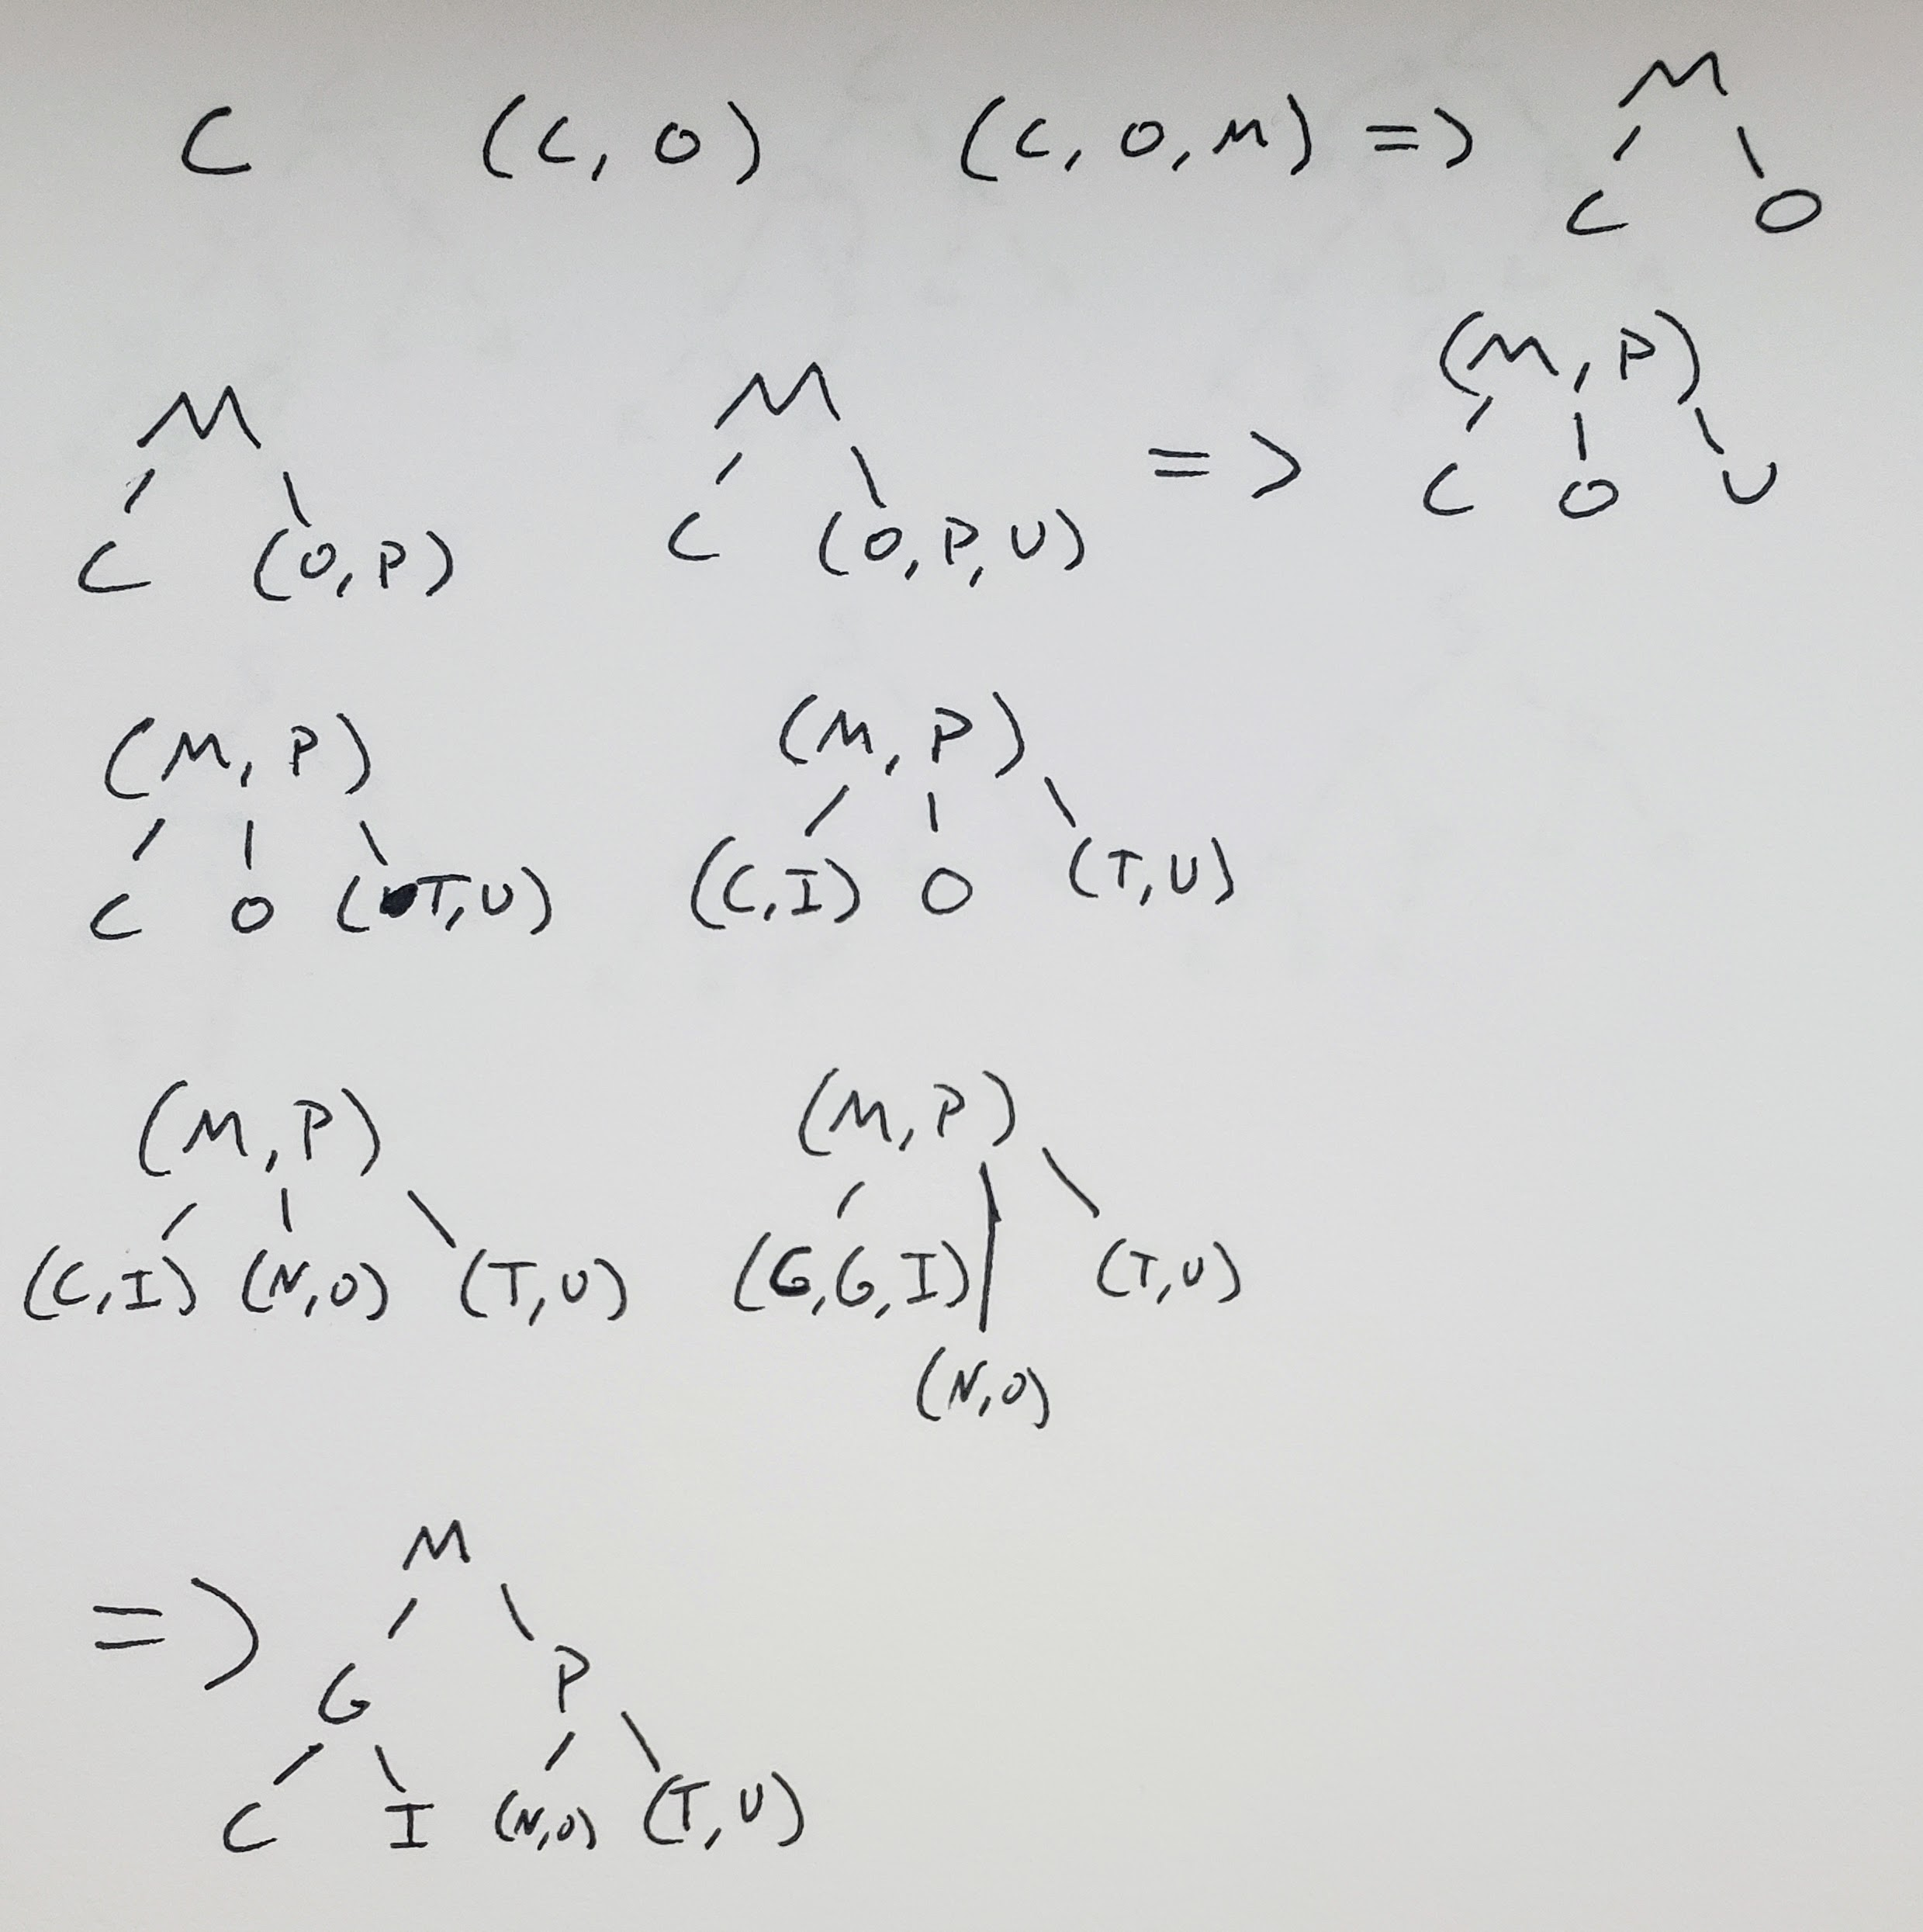
\includegraphics[width=\linewidth]{pics/num_5.jpg}
\end{figure}

\hwnumber{6(a)}
\begin{figure}[h!]
  \centering
  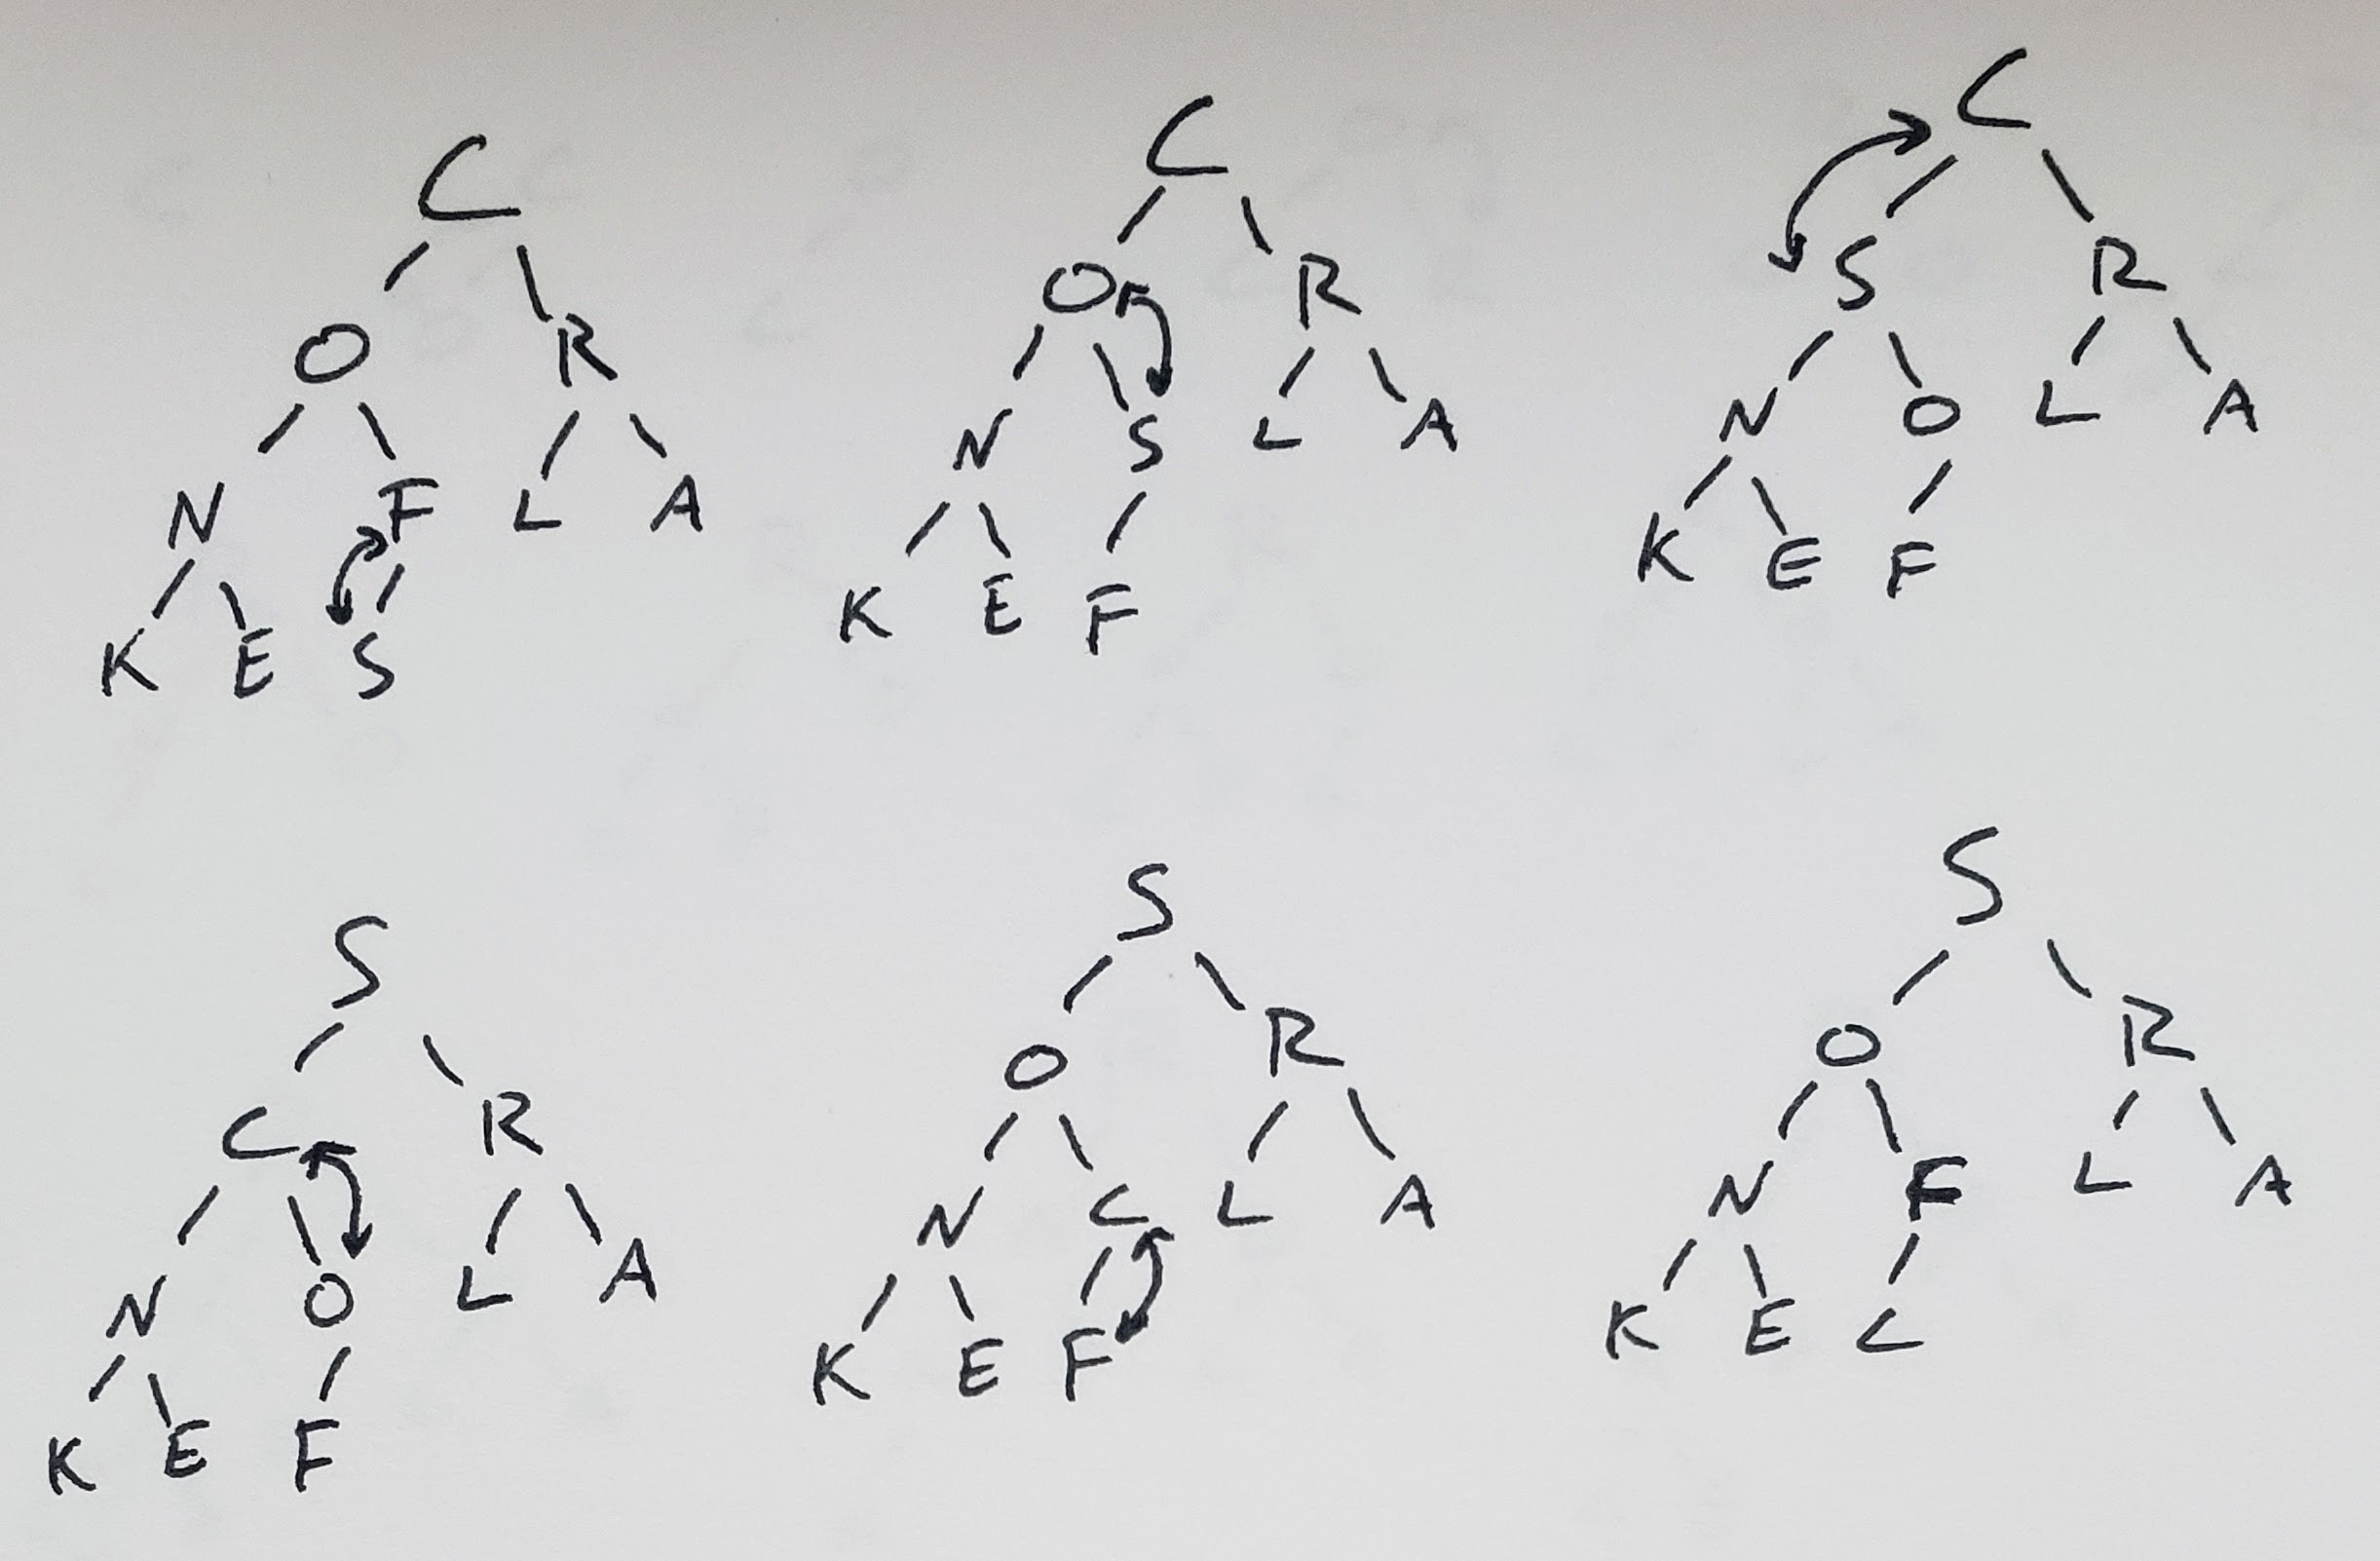
\includegraphics[width=\linewidth]{pics/num_6.jpg}
\end{figure}

\hwnumber{6(b)}
\begin{figure}[h!]
  \centering
  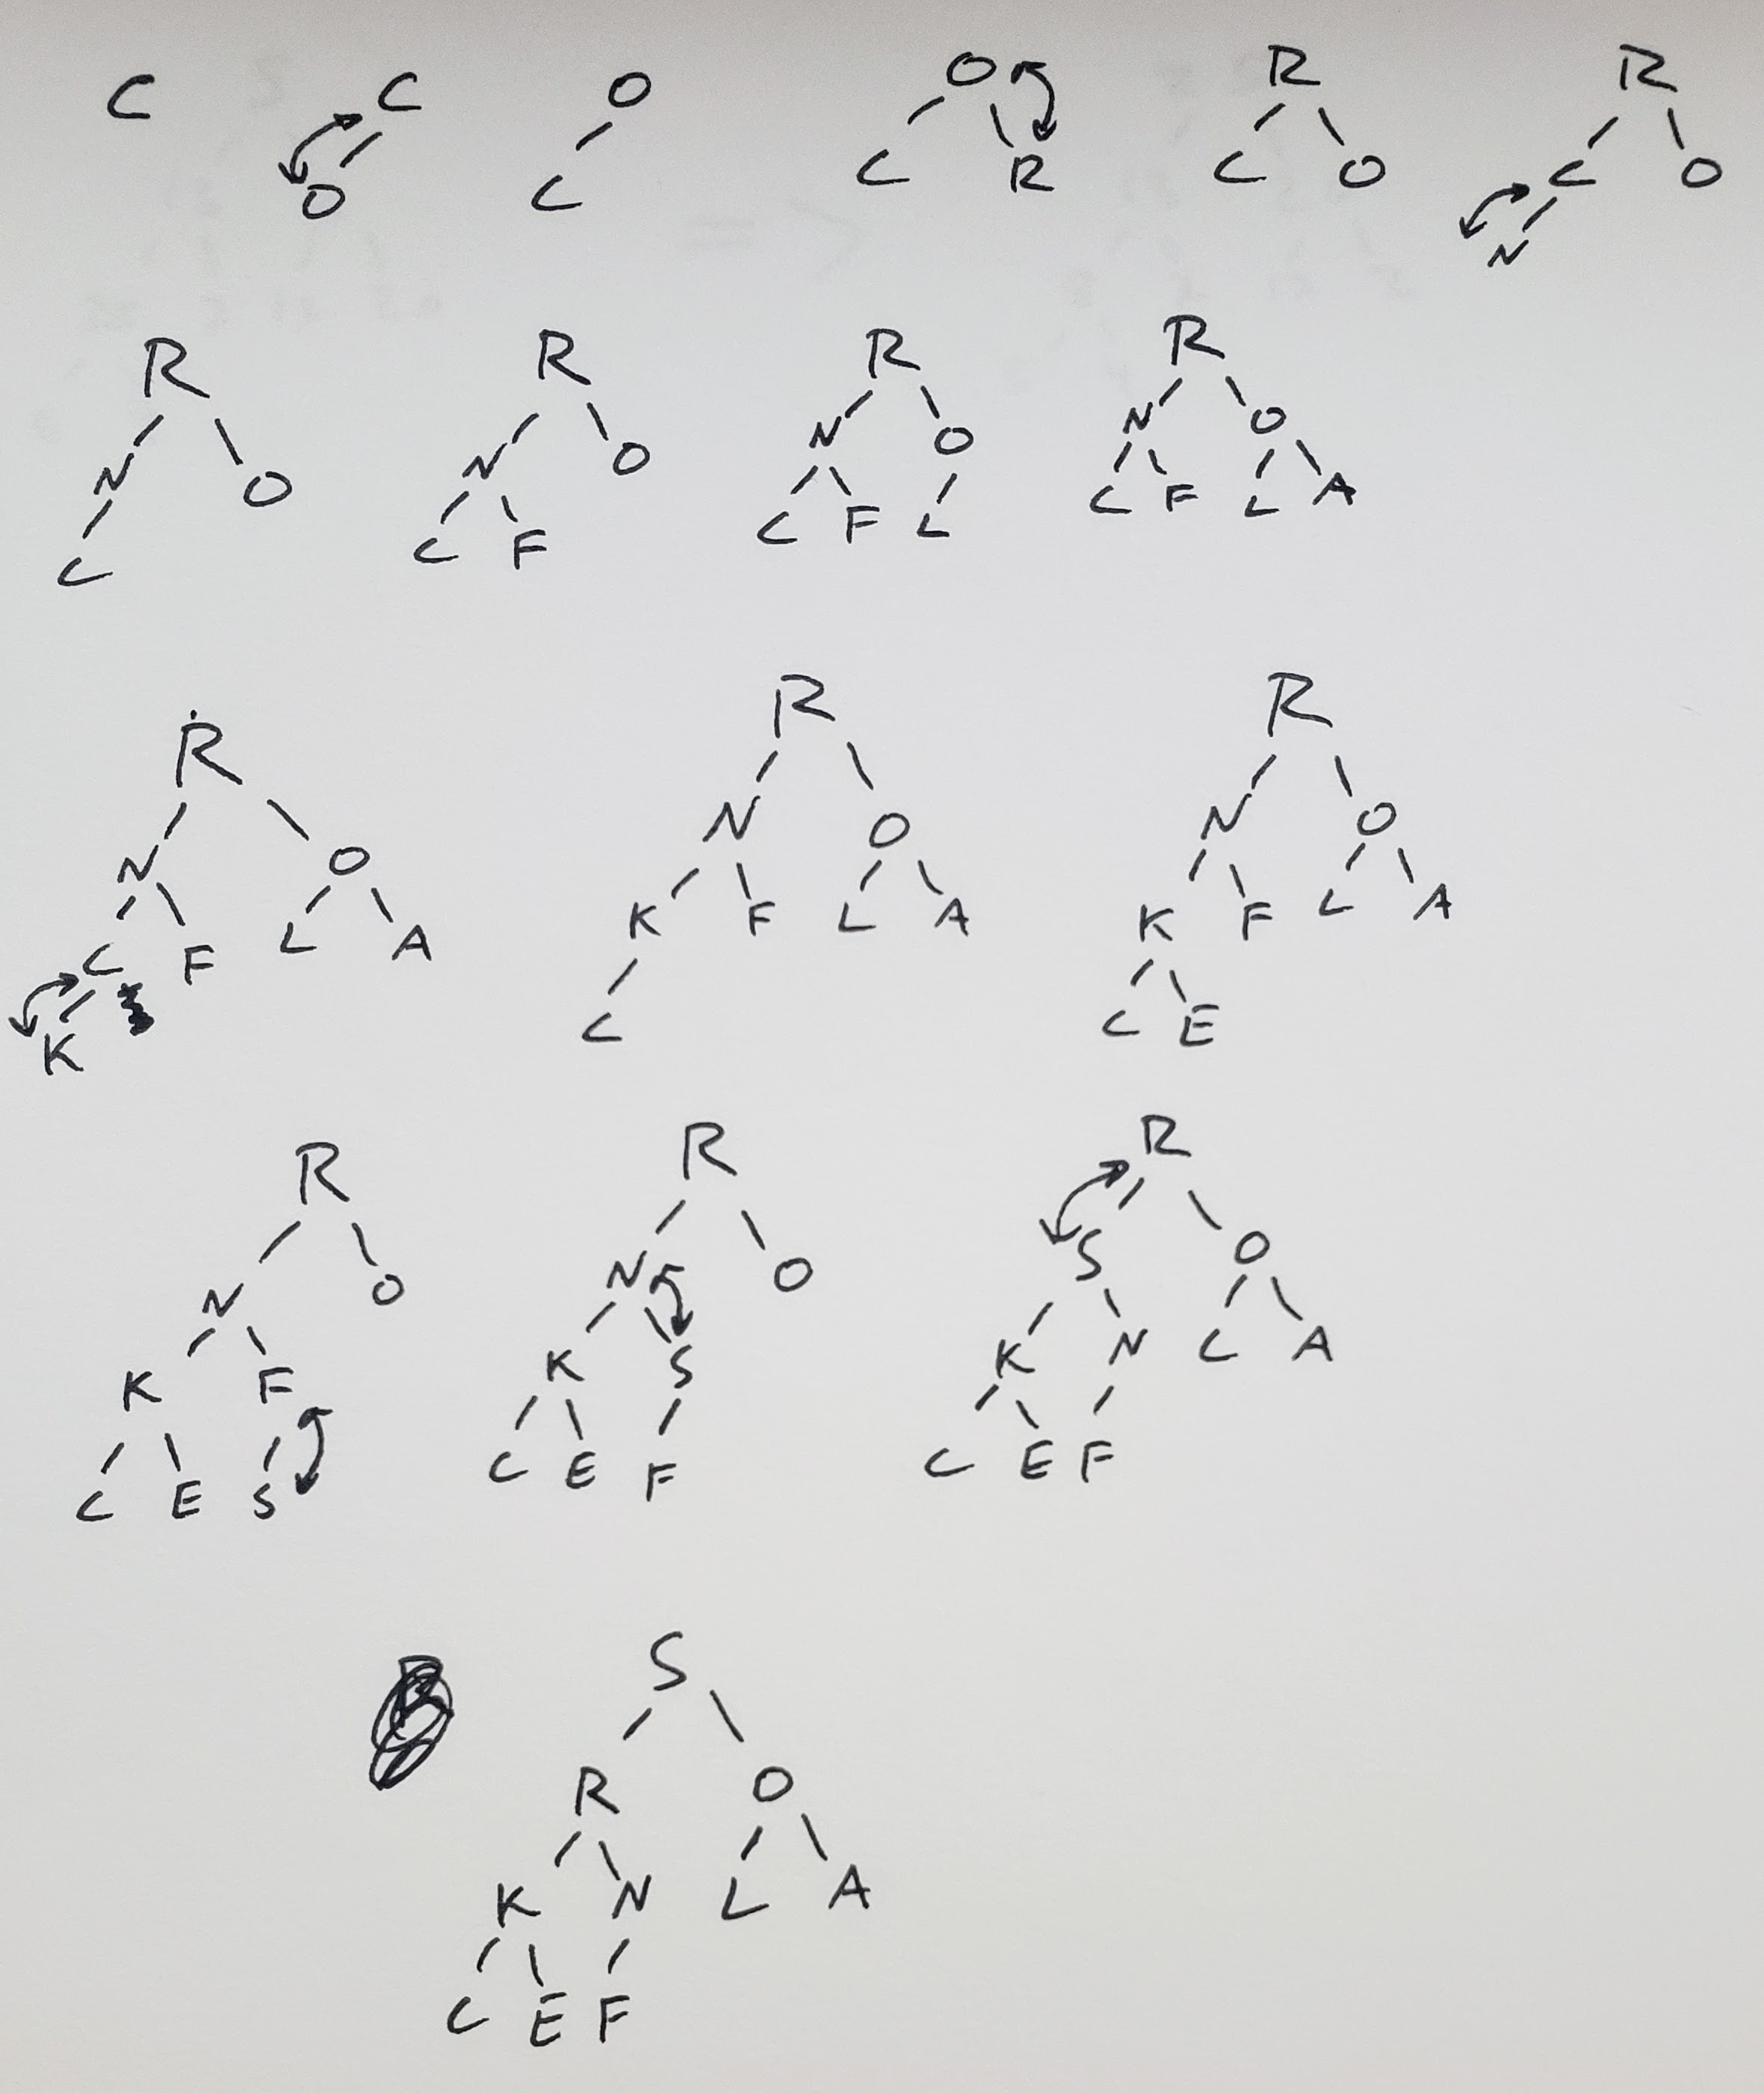
\includegraphics[width=\linewidth]{pics/num_6_b.jpg}
\end{figure}

\hwnumber{7}

First, we create the max heap, and then we proceed with the deleting procedure. 
\begin{figure}[h!]
  \centering
  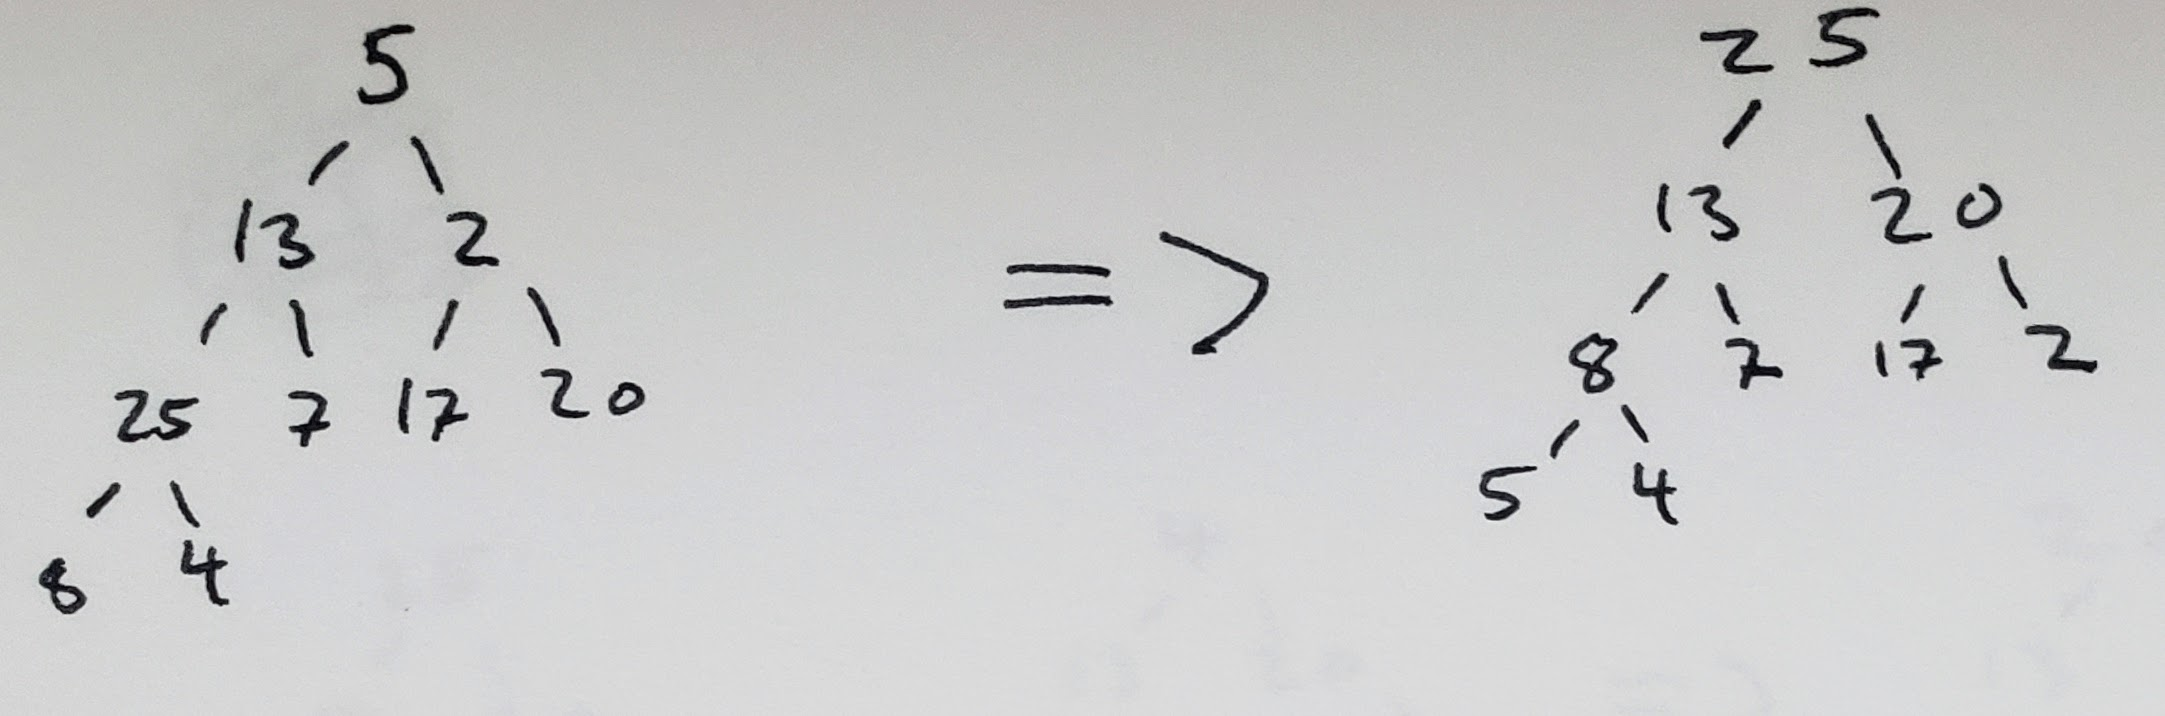
\includegraphics[width=\linewidth]{pics/num_7_first.jpg}
\end{figure}

\begin{figure}[h!]
  \centering
  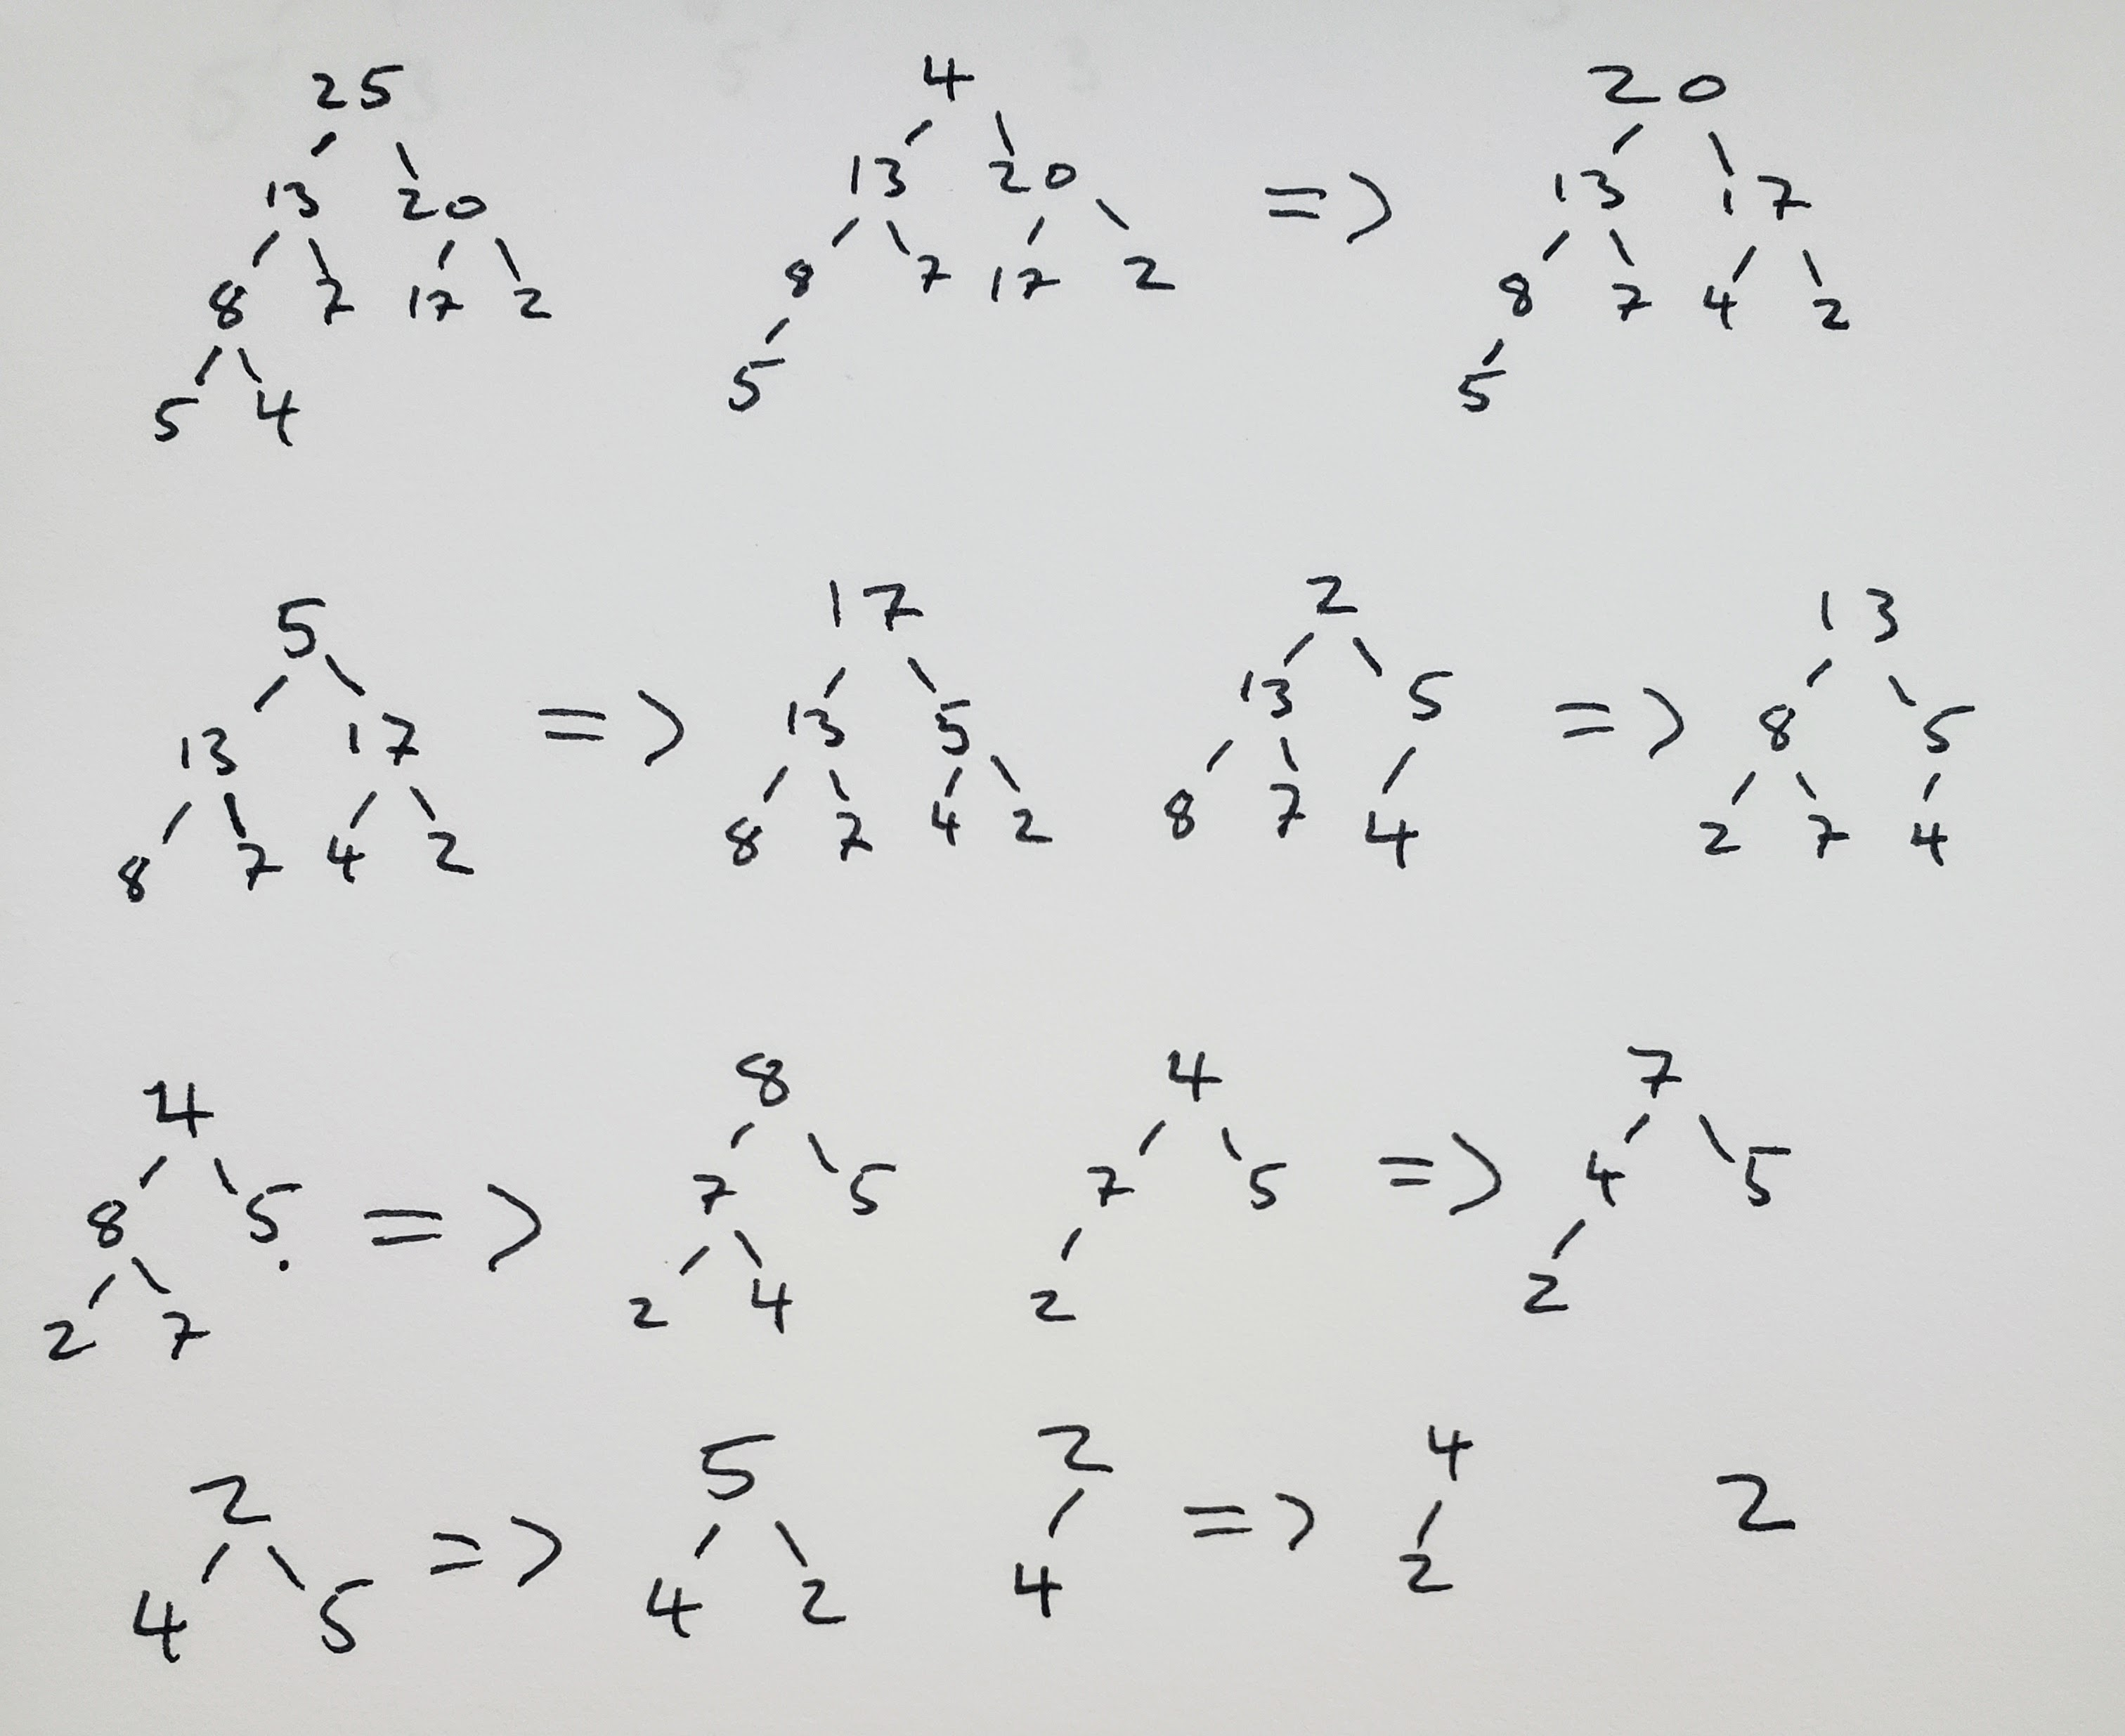
\includegraphics[width=\linewidth]{pics/num_7_second.jpg}
\end{figure}

\hwnumber{8}

A counterexample is if we want to sort the array 5, 5', 3, where we denote the
second 5 with 5'. 

\begin{figure}[h!]
  \centering
  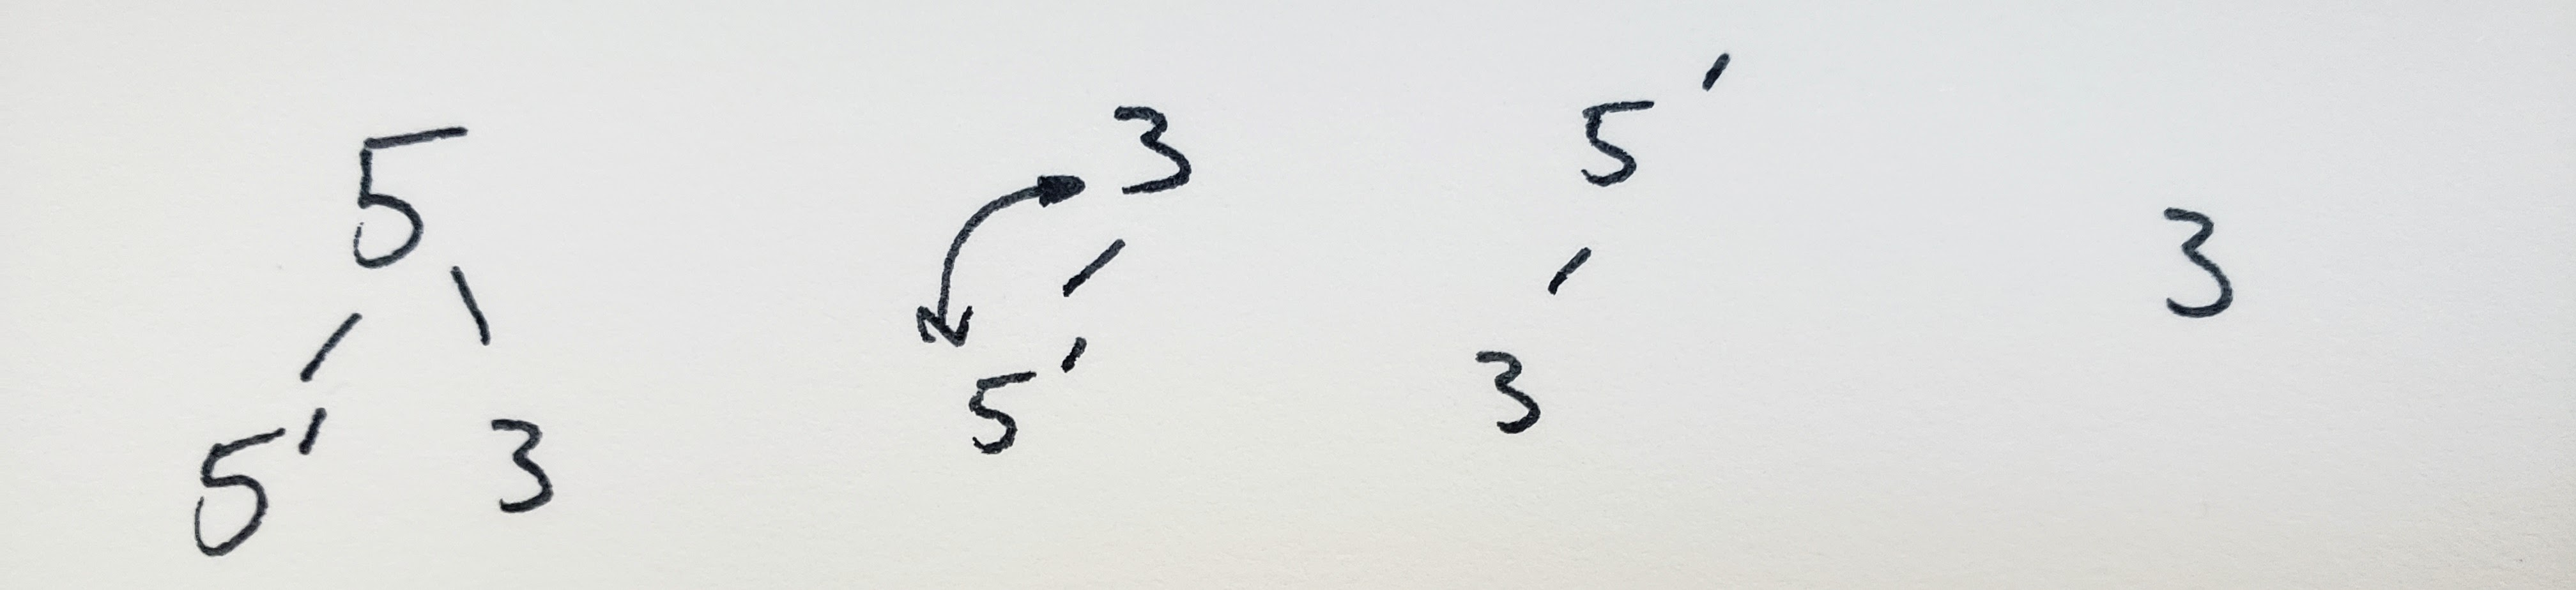
\includegraphics[width=\linewidth]{pics/num_8.jpg}
\end{figure}

Then the sorted array becomes 3, 5, 5'. So the two fives are swapped. 

\hwnumber{9}
\begin{figure}[h!]
  \centering
  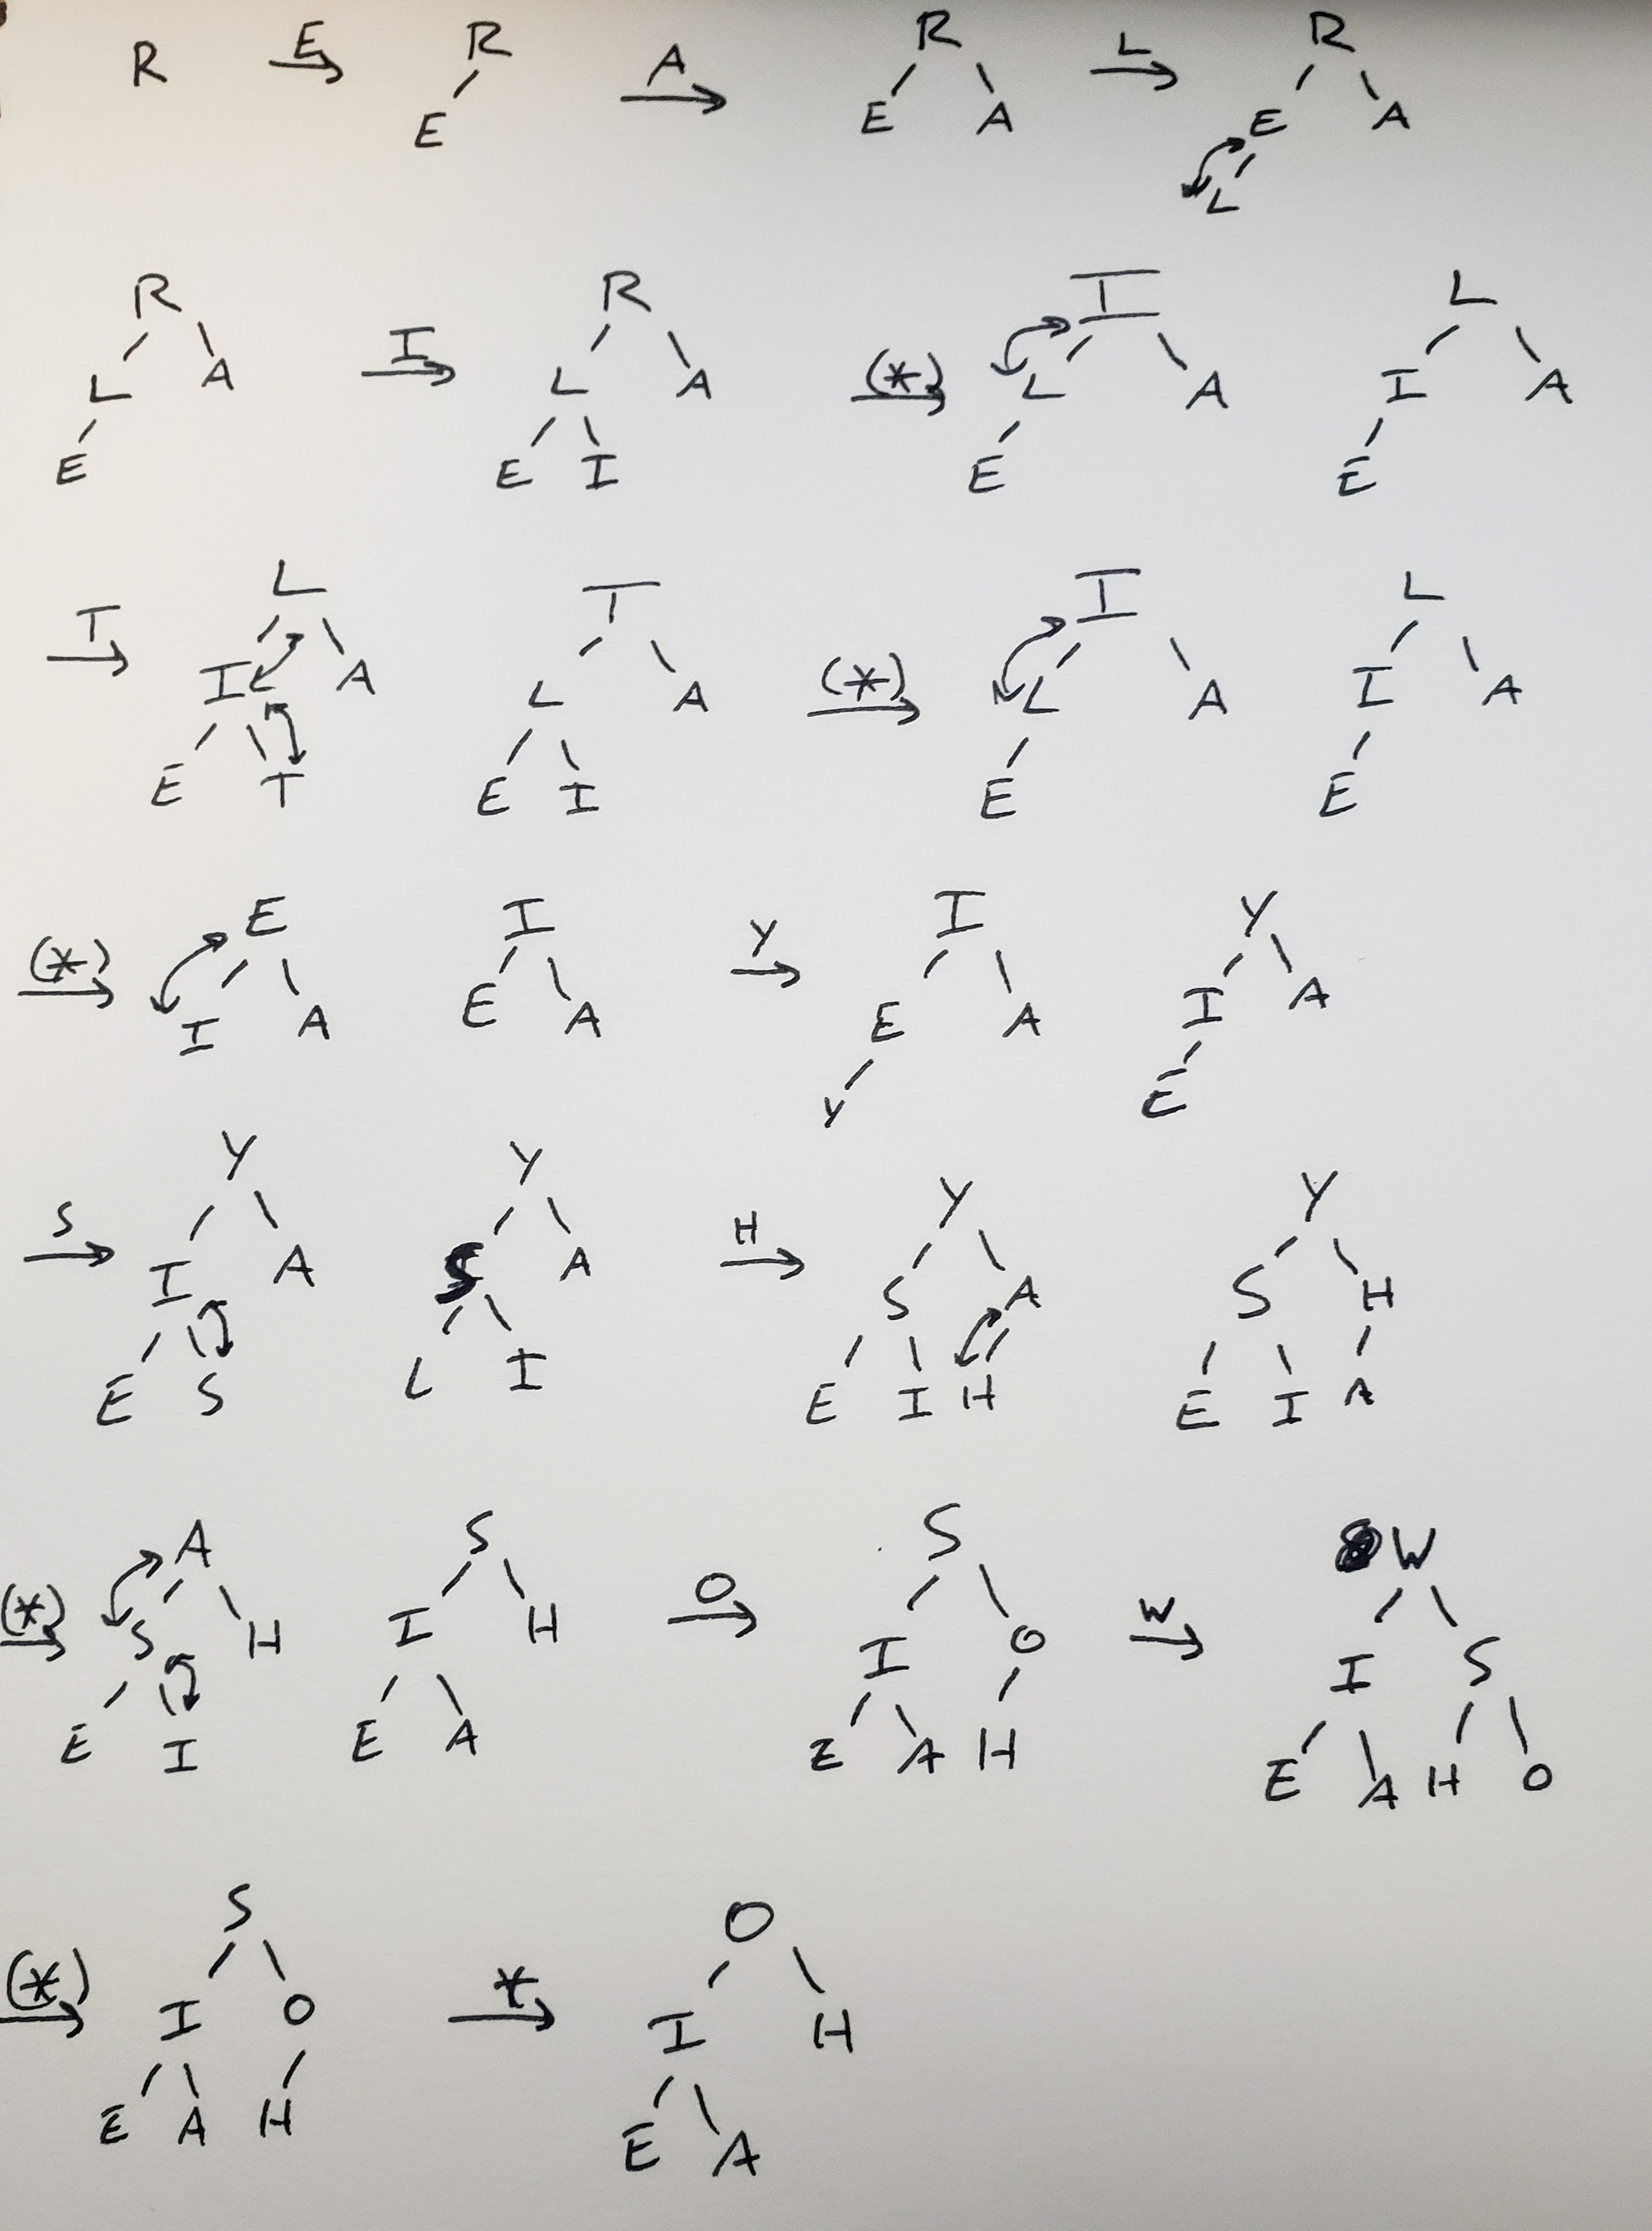
\includegraphics[width=\linewidth]{pics/num_9.jpg}
\end{figure}

\hwnumber{10}
The frequency and distribution arrays are as follows.

\begin{center}
  \begin{tabular}{l | c c c c}
    Array values & a & b & c & d\\
    \hline
    Frequency & 2 & 3 & 2 & 1\\
    Distribution & 2 & 5 & 7 & 8
  \end{tabular}
\end{center}

Then we build the sorted array.

\begin{center}
  \begin{tabular}{l | c c c c l | c | c | c | c | c | c | c | c |}
    & \multicolumn{4}{c}{\(D[0\dots 3]\)} & \multicolumn{8}{c}{Sorted array}\\
    \hline
    \\
    A[7] = b & 2 & 5 & 7 & 8 & &  &  &  &  & b &  &  &  \\
    A[6] = a & 2 & 4 & 7 & 8 & &  & a &  &  &  &  &  &  \\
    A[5] = a & 1 & 4 & 7 & 8 & & a &  &  &  &  &  &  &  \\
    A[4] = b & 0 & 4 & 7 & 8 & &  &  &  & b &  &  &  &  \\
    A[3] = c & 0 & 3 & 7 & 8 & &  &  &  &  &  &  & c &  \\
    A[2] = d & 0 & 3 & 6 & 8 & &  &  &  &  &  &  &  & d \\
    A[1] = c & 0 & 3 & 6 & 7 & &  &  &  &  &  & c &  &  \\
    A[0] = b & 0 & 3 & 5 & 7 & &  &  & b &  &  &  &  &  \\
  \end{tabular}
\end{center}

So the sorted array is a, a, b, b, b, c, c, d. 
\end{document}
